\documentclass[10pt]{beamer}
\usetheme[
%%% options passed to the outer theme
%    hidetitle,           % hide the (short) title in the sidebar
%    hideauthor,          % hide the (short) author in the sidebar
%    hideinstitute,       % hide the (short) institute in the bottom of the sidebar
%    shownavsym,          % show the navigation symbols
%    width=2cm,           % width of the sidebar (default is 2 cm)
%    hideothersubsections,% hide all subsections but the subsections in the current section
%    hideallsubsections,  % hide all subsections
    left               % right of left position of sidebar (default is right)
%%% options passed to the color theme
%    lightheaderbg,       % use a light header background
  ]{AAUsidebar}

% If you want to change the colors of the various elements in the theme, edit and uncomment the following lines
% Change the bar and sidebar colors:
%\setbeamercolor{AAUsidebar}{fg=red!20,bg=red}
%\setbeamercolor{sidebar}{bg=red!20}
% Change the color of the structural elements:
%\setbeamercolor{structure}{fg=red}
% Change the frame title text color:
%\setbeamercolor{frametitle}{fg=blue}
% Change the normal text color background:
%\setbeamercolor{normal text}{bg=gray!10}
% ... and you can of course change a lot more - see the beamer user manual.


\usepackage[utf8]{inputenc}
\usepackage[english]{babel}
\usepackage[T1]{fontenc}
% Or whatever. Note that the encoding and the font should match. If T1
% does not look nice, try deleting the line with the fontenc.
\usepackage{helvet}

\usepackage{listings} % Required for inserting code snippets

%Changing lis name from 'Listing' to 'Code Example'
\renewcommand{\lstlistingname}{Code Example}

%Defining colors used in our style
\definecolor{color3}{RGB}{230, 231, 231} % background
\definecolor{Blue}{RGB}{0, 51, 204} % keywords
\definecolor{Gray}{RGB}{153, 153, 153} % line numbers
\definecolor{PineGlade}{RGB}{204, 204, 153}

%Our style
\lstdefinestyle{Python1}{ 
language=Python,
frame=single,
basicstyle=\scriptsize\ttfamily,
backgroundcolor=\color{color3},
keywordstyle=\color{color1}\bf,
captionpos=b,
breakatwhitespace=false,
breaklines=true,
numbers=left, % Location of line numbers, can take the values of: none, left, right
numbersep=6pt, % Distance of line numbers from the code box
numberstyle=\tiny, % Style used for line numbers \color{Gray}
commentstyle=\usefont{T1}{pcr}{m}{sl}\color{color1}
} 

\newcommand{\insertcodefile}[2]{\lstinputlisting[caption=#2,label=#1,style=Python1,float=h,belowskip=-0.8\baselineskip]{codeRelated/scripts/#1}} % The first argument is the script location/filename and the second is a caption for the code

\newcommand{\insertcodefileline}[4]{\begin{itemize}\item[]\lstinputlisting[firstnumber=#3,firstline=#3,lastline=#4,caption=#2,label=#1,style=Python1]{codeRelated/scripts/#1}\end{itemize}}

%----------------------------------------------------------------------------------------
%ALDRIG KALD DENNE STYLE!!!!!!!!!!!!!!!!!!!!!, kun her som reference til hvordan vi laver vores egen.
%----------------------------------------------------------------------------------------

\lstdefinestyle{Style1}{ % Define a style for your code snippet, multiple definitions can be made if, for example, you wish to insert multiple code snippets using different programming languages into one document
language=Python, % Detects keywords, comments, strings, functions, etc for the language specified
backgroundcolor=\color{highlight}, % Set the background color for the snippet - useful for highlighting
basicstyle=\footnotesize\ttfamily, % The default font size and style of the code
breakatwhitespace=false, % If true, only allows line breaks at white space
breaklines=true, % Automatic line breaking (prevents code from protruding outside the box)
captionpos=b, % Sets the caption position: b for bottom; t for top
commentstyle=\usefont{T1}{pcr}{m}{sl}\color{DarkGreen}, % Style of comments within the code - dark green courier font
deletekeywords={}, % If you want to delete any keywords from the current language separate them by commas
%escapeinside={\%}, % This allows you to escape to LaTeX using the character in the bracket
%firstnumber=1, % Line numbers begin at line 1
frame=single, % Frame around the code box, value can be: none, leftline, topline, bottomline, lines, single, shadowbox
frameround=tttt, % Rounds the corners of the frame for the top left, top right, bottom left and bottom right positions
keywordstyle=\color{Blue}\bf, % Functions are bold and blue
morekeywords={}, % Add any functions no included by default here separated by commas
numbers=left, % Location of line numbers, can take the values of: none, left, right
numbersep=10pt, % Distance of line numbers from the code box
numberstyle=\tiny\color{Gray}, % Style used for line numbers
rulecolor=\color{black}, % Frame border color
showstringspaces=false, % Don't put marks in string spaces
showtabs=false, % Display tabs in the code as lines
stepnumber=1, % The step distance between line numbers, i.e. how often will lines be numbered
stringstyle=\color{Purple}, % Strings are purple
tabsize=2, % Number of spaces per tab in the code
}


% colored hyperlinks
\newcommand{\chref}[2]{%
  \href{#1}{{\usebeamercolor[bg]{AAUsidebar}#2}}%
}

\title[SkiRaff an ETL Testing Framework for pygrametl]% optional, use only with long paper titles
{SkiRaff an ETL Testing Framework for pygrametl}

\subtitle{}  % could also be a conference name

\date{\today}

\author[Alexander Branborg,\\ Arash Michael Sami Kjær,\\ Mathias Claus Jensen,\\  Mikael Vind Mikkelsen] % optional, use only with lots of authors
{
	Alexander Branborg \href{abran13@student.aau.dk}{{\tt abran13@student.aau.dk}}\\
	Arash Michael Sami Kjær \href{ams13@student.aau.dk}{{\tt ams13@student.aau.dk}}\\
	Mathias Claus Jensen \href{mcje13@student.aau.dk}{{\tt mcje13@student.aau.dk}}\\
  Mikael Vind Mikkelsen \href{mvmi12@student.aau.dk}{{\tt mvmi12@student.aau.dk}}
}
% - Give the names in the same order as they appear in the paper.
% - Use the \inst{?} command only if the authors have different
%   affiliation. See the beamer manual for an example

\institute[
%  {\includegraphics[scale=0.2]{aau_segl}}\\ %insert a company, department or university logo
  Department of Computer Science\\
  Aalborg University\\
  Denmark
] % optional - is placed in the bottom of the sidebar on every slide
{% is placed on the title page
  Department of Computer Science\\
  Aalborg University\\
  Denmark
  
  %there must be an empty line above this line - otherwise some unwanted space is added between the university and the country (I do not know why;( )
}


% specify a logo on the titlepage (you can specify additional logos an include them in 
% institute command below
\pgfdeclareimage[height=1.5cm]{titlepagelogo}{AAUgraphics/aau_logo_new} % placed on the title page
%\pgfdeclareimage[height=1.5cm]{titlepagelogo2}{graphics/aau_logo_new} % placed on the title page
\titlegraphic{% is placed on the bottom of the title page
  \pgfuseimage{titlepagelogo}
%  \hspace{1cm}\pgfuseimage{titlepagelogo2}
}


\begin{document}
% the titlepage
{\aauwavesbg%
\begin{frame}[plain,noframenumbering] % the plain option removes the sidebar and header from the title page
  \titlepage
\end{frame}}
%%%%%%%%%%%%%%%%

% TOC
\begin{frame}{Agenda}{}
\tableofcontents
\end{frame}
%%%%%%%%%%%%%%%%

%\section{Introduction}
% motivation for creating this theme
\begin{frame}{Introduction}{}
  The present beamer theme called the \alert{AAU Sidebar Beamer Theme} is an attempt to
  \begin{itemize}
    \item<1-> create a simple and elegant beamer theme which can be used by students and researchers affiliated with Aalborg University (AAU),
    \item<2-> create a unique AAU theme which does not resemble any of the standard beamer themes. People should associate this theme with AAU and not with beamer,
    \item<3-> keep the amount of clutter to a minimum. Only the important things should be on the slides,
    \item<4-> retain the powerful customisation tools provided by the template system of the beamer class.
  \end{itemize}
\end{frame}
%%%%%%%%%%%%%%%%

\subsection{License}
% the license
\begin{frame}{Introduction}{License}
  \begin{itemize}
    \item<1-> The AAU logo is covered by copyright rules. I have used the logo from \chref{http://aau.designguides.dk}{http://aau.designguides.dk}. As long as you use the theme for making presentations in connection with your work at AAU, you are allowed to use the AAU logo.
    \item<2-> The rest of the theme is provided under the GNU General Public License v. 3 (GPLv3). This basically means that you can redistribute it and/or modify it under the same license. For more information on the GPL license see \chref{http://www.gnu.org/licenses/}{http://www.gnu.org/licenses/}
  \end{itemize}
\end{frame}
%%%%%%%%%%%%%%%%

\section{Installation}
% general installation instructions
\begin{frame}{Installation}
  The theme consists of four files
  \begin{enumerate}
    \item {\tt beamerthemeAAUsidebar.sty}
    \item {\tt beamerinnerthemeAAUsidebar.sty}
    \item {\tt beamerouterthemeAAUsidebar.sty}
    \item {\tt beamercolorthemeAAUsidebar.sty}
  \end{enumerate}
  The theme can either be installed for local or global use.
  \pause
  \begin{block}{Local Installation}
    The simplest way of installing the theme is by placing the four theme files in the same folder as your presentation. When you download the theme, the four theme files are located in the {\tt local} folder.
  \end{block}
\end{frame}

% general installation instructions
\begin{frame}{Installation}
  \begin{block}{Global Installation}
  \begin{itemize}
     \item If you wish to make the theme globally available, you must put the files in your local latex directory tree. The location of the root of the local directory tree depends on the operating system and the latex distribution. On the following slides, you can read the instructions for some common setups.
    \item When you download the theme, the four theme files are embedded in a directory structure (in the {\tt global} folder) ready to be copied directly to the root of your local directory tree.
    \item On the following slides, we refer to this directory structure as {\tt <dirstruct>}. \alert{Note} that some parts of the directory may already exist if you have installed other packages in your local latex directory tree. If this is the case, you simply merge {\tt <dirstruct>} with your existing setup.
  \end{itemize}
  \end{block}
\end{frame}

\subsection{GNU/Linux}
% installation on GNU/Linux
\begin{frame}{Installation}{GNU/Linux}
  \begin{block}{Ubuntu with TeX Live}
    \begin{enumerate}
      \item Place the {\tt <dirstruct>} in the root of your local latex directory tree. By default it is\\
        {\tt \textasciitilde /texmf}\\
        If the root does not exist, create it. The symbol {\tt \textasciitilde} refers to your home folder, i.e., {\tt /home/<username>}
      \item In a terminal run\\
        {\tt \$ texhash \textasciitilde /texmf}
    \end{enumerate}
  \end{block}
\end{frame}
%%%%%%%%%%%%%%%%

\subsection{Microsoft Windows}
% installation on Microsoft Windows
\begin{frame}{Installation}{Microsoft Windows}
  \begin{block}{Windows with MiKTeX}
    Apparently, MiKTeX does not include a local latex directory tree by default. Therefore, you first have to create it.
    \begin{enumerate}
      \item To do this, create a folder {\tt <somewhere>} named, e.g., {\tt texmf}
      \item Add this folder in the Roots tab of the MiKTeX Settings dialog
      \item Place the {\tt <dirstruct>} in your newly created local latex directory tree\\
    {\tt <somewhere>\textbackslash texmf}\\
      \item Open the MiKTeX Settings dialog and click Refresh FNDB.
    \end{enumerate}
  \end{block}
\end{frame}
%%%%%%%%%%%%%%%%

% installation on Microsoft Windows Cont'd
\begin{frame}{Installation}{Microsoft Windows}
  \begin{block}{Windows with TeX Live}
    In the advanced TeX Live Installer, you can manually change the default position of the root of the local latex directory tree. However, we assume the default position below.
    \begin{enumerate}
      \item Place the {\tt <dirstruct>} in your local latex directory tree\\
        {\tt \%USERPROFILE\%\textbackslash texmf}\\
        If it does not exist, create it. In XP {\tt \%USERPROFILE\%} is\\
      {\tt c:\textbackslash Document and Settings\textbackslash<username>}\\
      by default, and in Vista and above it is by default\\
      {\tt c:\textbackslash Users\textbackslash<username>}
      \item Open the TeX Live Manager dialog and select 'Update filename database' under 'Actions'.
    \end{enumerate}
  \end{block}
\end{frame}
%%%%%%%%%%%%%%%%

\subsection{Mac OS X}
% installation on Mac OS X
\begin{frame}{Installation}{Mac OS X}
  \begin{block}{Mac OS X with MacTeX}
     Place the {\tt <dirstruct>} in the root of your local latex directory tree. By default it is\\
        {\tt \textasciitilde /Library/texmf}\\
        If the root does not exist, create it. The symbol {\tt \textasciitilde} refers to your home folder, i.e., {\tt /home/<username>}
  \end{block}
\end{frame}
%%%%%%%%%%%%%%%%

\subsection{Required Packages}
% list of required packages
\begin{frame}{Installation}{Required Packages}
  Of course, you have to have the Beamer class installed. In addition, the theme loads two packages
  \begin{itemize}
    \item TikZ\footnote{By the way, TikZ is an awesome package for creating beautiful graphics. If you do not believe me, then have a look at these \chref{http://www.texample.net/tikz/examples/}{online examples} or the \chref{http://tug.ctan.org/tex-archive/graphics/pgf/base/doc/generic/pgf/pgfmanual.pdf}{pgf user manual}. If you want to create beautiful plots, you should use the pgfplots package which is based on TikZ.}
    \item calc
  \end{itemize}
  These packages are very common and should therefore be included in your latex distribution.
\end{frame}
%%%%%%%%%%%%%%%%

\section{User Interface}
\subsection{Loading the Theme and Theme Options}
% list of the themes and options
\begin{frame}{User Interface}{Loading the Theme and Theme Options}
  \begin{block}{The Presentation Theme}
    It is very simple to load the presentation theme. Just type\\
    {\tt \textbackslash usetheme[<options>]\{AAUsidebar\}}\\
    which is exactly the same way other beamer presentation themes are loaded. The presentation theme loads the inner, outer and color AAU sidebar theme files and passes the {\tt <options>} on to these files.
  \end{block}
  \begin{block}{The Inner Theme}
    You can load the inner theme directly by\\
    {\tt \textbackslash useinnertheme\{AAUsidebar\}}\\
    and it has no options.
  \end{block}
\end{frame}
%%%%%%%%%%%%%%%%

% list of the themes and options
\begin{frame}{User Interface}{Loading the Theme and Theme Options}
  \begin{block}{The Outer Theme}
    You can load the outer theme directly by\\
    {\tt \textbackslash useoutertheme[<options>]\{AAUsidebar\}}\\
    Currently, the theme options are
  \begin{itemize}
    \item {\tt hidetitle}: Hide the (short) title in the sidebar
    \item {\tt hideauthor}: hide the (short) author in the sidebar
    \item {\tt hideinstitute}: hide the (short) institute in the bottom of the sidebar
    \item {\tt shownavsym}: show the navigation symbols
    \item {\tt left} or {\tt right}: position of the sidebar (default is right)
    \item {\tt width=<length>}: width of the sidebar (default is 2 cm).
    %The width is measured from the right side of the vertical bar to the right edge of the slide.
    \item {\tt hideothersubsections}: hide all subsections but the subsections in the current section
    \item {\tt hideallsubsections}: hide all subsections
  \end{itemize}
  The last four options are inherited from the outer sidebar theme.
  \end{block}
\end{frame}
%%%%%%%%%%%%%%%%

% list of the themes and options
{\setbeamercolor{frametitle}{use=structure,fg=structure.fg,bg=white}
\begin{frame}{User Interface}{Loading the Theme and Theme Options}
  \begin{block}{The Color Theme}
    You can load the color theme directly by\\
    {\tt \textbackslash usecolortheme[<options>]\{AAUsidebar\}}\\
    Currently, the only theme option is
    \begin{itemize}
      \item {\tt lightheaderbg}: use a light header background (currently, it is white). 
    \end{itemize}
    This option creates the light header used on this slide.
  \end{block}
  \pause
  \begin{block}{The Color Element {\tt AAUsidebar}}
    The color theme defines a new beamer color element named {\tt AAUsidebar} whose foreground and background colors are
    \begin{itemize}
      \item fg: {\usebeamercolor[fg]{AAUsidebar}light blue (\{RGB\}\{194,193,204\})}
      \item bg: {\usebeamercolor[bg]{AAUsidebar}dark blue (\{RGB\}\{33,26,82\})}
    \end{itemize}
    You can use these colors in the standard beamer way by using the command
    {\tt \textbackslash usebeamercolor[<fg or bg>]\{AAUsidebar\}}. See the beamer manual for instructions.
  \end{block}
\end{frame}
}
%%%%%%%%%%%%%%%%

\subsection{Compilation}
% compilation
\begin{frame}{User Interface}{Compilation}
\begin{block}{Compiling Your Presentation With the AAU Sidebar Theme}
  Unlike most other beamer themes, this theme must be compiled at least \alert{three} times to make everything look right. For most other themes, you do not have to compile your presentation more than two times. For the AAU sidebar theme, the third compilation is necessary to determine the position of the circle with the current frame number.
\end{block}
\end{frame}
%%%%%%%%%%%%%%%%

\subsection{Modifying the Theme}
% how to modify the theme
{\setbeamercolor{AAUsidebar}{fg=gray!50,bg=gray}
 \setbeamercolor{sidebar}{bg=red!20}
 \setbeamercolor{structure}{fg=red}
 \setbeamercolor{frametitle}{use=structure,fg=structure.fg,bg=red!5}
 \setbeamercolor{normal text}{bg=gray!20}
\begin{frame}{User Interface}{Modifying the Theme}
  \begin{itemize}
    \item<1-> The default configuration of fonts, colors, and layout complies with the \chref{http://aau.designguides.dk}{AAU design guidelines} and is the \alert{official} version of the theme.
    \item<2-> However, you can easily modify specific elements of the theme through the template system provided by the beamer class. Please refer to the beamer user manual for instructions.
    \item<3-> For example, on this slide we have used
      \begin{itemize}
        \item Change the sidebar colors:\\
        {\tt \textbackslash setbeamercolor\{AAUsidebar\}\{fg=gray!50,bg=gray\}}
        {\tt \textbackslash setbeamercolor\{sidebar\}\{bg=red!20\}}
        \item Change the color of the structural elements:\\
        {\tt \textbackslash setbeamercolor\{structure\}\{fg=red\}}\\
        \item Change the frame title text color and background:
        {\tt \textbackslash setbeamercolor\{frametitle\}\{use=structure, fg=structure.fg,bg=red!5\}}
        \item Change the background color of the text
        {\tt \textbackslash setbeamercolor\{normal text\}\{bg=gray!20\}}
      \end{itemize}
  \end{itemize}
\end{frame}}
%%%%%%%%%%%%%%%%

\subsection{AAU Waves}
% the AAU Waves background
\begin{frame}{User Interface}{The AAU Waves Background Image}
\begin{block}{The AAU Waves Background Image}
\begin{itemize}
  \item<1-> In this documentation, the title page frame and the last frame have the AAU waves as the background image. The AAU waves background image can be added to any single frame by wrapping a frame in the following way\\
  {\tt \{\textbackslash aauwavesbg\\
    \textbackslash begin\{frame\}[<options>]\{Frame Title\}\{Frame Subtitle\}\\
    \ldots\\
    \textbackslash end\{frame\}\}}
  \item<2-> Ideally, I would like to create a new frame option called {\tt aauwavesbg} which can enable the AAU waves background. However, I have not been able to figure out how such an option can be added. If you know how this can be done, please contact me.
\end{itemize}
\end{block}
\end{frame}
%%%%%%%%%%%%%%%%

\subsection{Widescreen Support}
% Widescreen Support
\begin{frame}{User Interface}{Widescreen Support}
\begin{block}{Widescreen Support}
  Newer projectors and almost any modern TV support a widescreen format such as 16:10 or 16:9. Beamer (>= v. 3.10) supports various aspect ratios of the slides. According to section 8.3 on page 77 of the Beamer user guide v. 3.10, you can write\\
{\tt\textbackslash documentclass[aspectratio=1610]\{beamer\}}\\
to get slides with an aspect ratio of 16:10. You can also use 169, 149, 54, 43 (default), and 32 to get other aspect ratios.
\end{block}
\end{frame}
%%%%%%%%%%%%%%%%

\section{Feedback}
\subsection{Known Problems}
% known problems
\begin{frame}{Feedback}{Known Problems}
  \begin{description}
    \item[Overlapping footnote] You might have problems with a too wide footnote text width. This is problem with older versions of Beamer, and it can be resolved by updating Beamer to a newer version. You can read more about it in \chref{https://bitbucket.org/rivanvx/beamer/issue/200/width-of-footnote-in-a-sidebar-theme}{this bugreport}.
  \end{description}
\end{frame}
%%%%%%%%%%%%%%%%

\subsection{Bugs, Comments and Suggestions}
% help me iron out the bugs or give me some comment and suggestions
\begin{frame}{Feedback}{Bugs, Comments and Suggestions}
  \begin{itemize}
    \item<1-> There are probably still a lot of bugs in the theme. If you should find one, then please let me know. No bug is too small!
    \item<2-> Also, please contact me, if you have some exciting new ideas or just some simple usability improvements.
  \end{itemize}
\end{frame}
%%%%%%%%%%%%%%%%
\section{Mathias}
% motivation for creating this theme
\begin{frame}{Mathias}{}
  Mathias
  \begin{itemize}
    \item<1-> Mathias 1
    \item<2-> Mathias 2
    \item<3-> Mathias 3
    \item<4-> Mathias 4
  \end{itemize}
\end{frame}
%%%%%%%%%%%%%%%%
\section{Arash}
% motivation for creating this theme
\begin{frame}{Arash}{}
  Arash
  \begin{itemize}
    \item<1-> Arash 1
    \item<2-> Arash 2
    \item<3-> Arash 3
    \item<4-> Arash 4
  \end{itemize}
\end{frame}
%%%%%%%%%%%%%%%%
%Predicates
%	Vis dem alle
%		Men snak kun om de seje
%		Func dep
%		Referential integrity
%		Compare
%	Vis kode for dem
%Hvorfor er de nyttige og hvordan løser de vores problem
%Hvordan anvendes de
%Alternativ implementering/design
%Andre nyttige predicates - Har vi covered enough

\section{Predicates}
%Nævn assertion af DW properties
\subsection{Hvorfor er de nyttige?}
\begin{frame}{Predicates}{Hvorfor er de nyttige?}
	\begin{itemize}
		\item<1-> Source to target test
		\item<1->[] 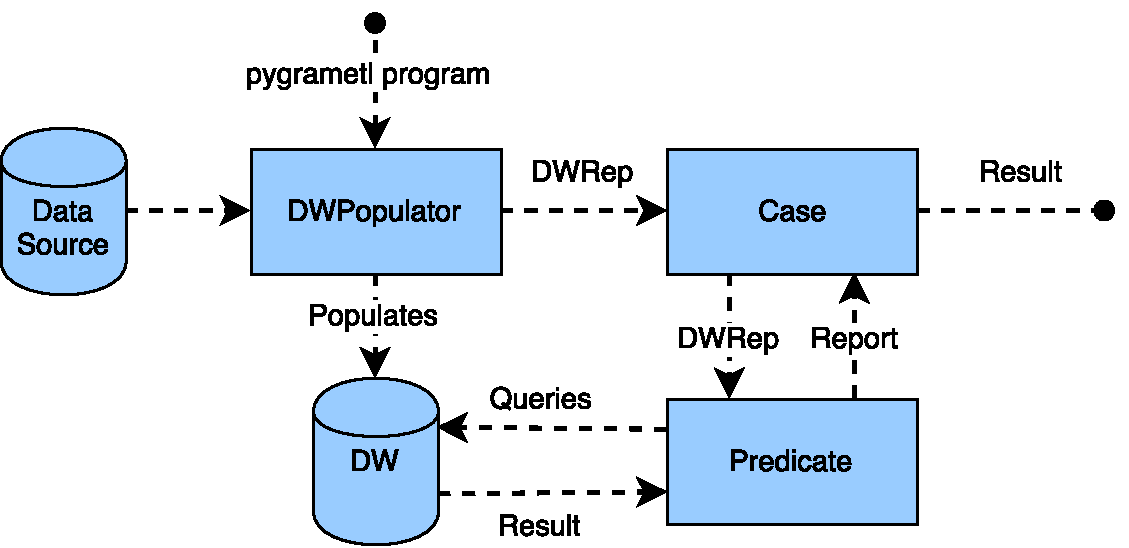
\includegraphics[width=8.5cm]{figures/overview.pdf}
		\item<2-> Regression testing
		\item<3-> Business Rules
	\end{itemize}
\end{frame}

\begin{frame}{Predicates}{Hvorfor er de nyttige?}
	\begin{block}{Predicates til rådighed i SKiRaff}
		\begin{itemize}
			\item<1-> RowCountPredicate
			\item<1-> ColumnNotNullPredicate
			\item<1-> ReferentialIntegrityPredicate
			\item<1-> FunctionalDependencyPredicate
			\item<1-> SCDVersionPredicate
			\item<1-> CompareTablePredicate
			\item<1-> RuleRowPredicate
			\item<1-> RuleColumnPredicate
		\end{itemize}
	\end{block}
\end{frame}

\begin{frame}{Predicates}{Hvorfor er de nyttige?}
	\begin{block}{Predicates til rådighed i SKiRaff}
		\begin{itemize}
			\item<1-> RowCountPredicate
			\item<1-> ColumnNotNullPredicate
			\item<1-> ReferentialIntegrityPredicate
			\item<1-> \textbf{FunctionalDependencyPredicate}
				\begin{itemize}
					\item<1-> \textbf{Har meget til fælles med mange af vores predicater.}
				\end{itemize}			
			\item<1-> SCDVersionPredicate
			\item<1-> CompareTablePredicate
			\item<1-> RuleRowPredicate
			\item<1-> RuleColumnPredicate
		\end{itemize}
	\end{block}
\end{frame}

\begin{frame}{Predicates}{Hvorfor er de nyttige?}
	\begin{block}{Predicates til rådighed i SKiRaff}
		\begin{itemize}
			\item<1-> RowCountPredicate
			\item<1-> ColumnNotNullPredicate
			\item<1-> \textbf{ReferentialIntegrityPredicate}
				\begin{itemize}
					\item<1-> \textbf{Advanceret predicate}
				\end{itemize}
			\item<1-> \textbf{FunctionalDependencyPredicate}
				\begin{itemize}
					\item<1-> \textbf{Har meget til fælles med mange af vores predicater.}
				\end{itemize}			
			\item<1-> SCDVersionPredicate
			\item<1-> CompareTablePredicate
			\item<1-> RuleRowPredicate
			\item<1-> RuleColumnPredicate
		\end{itemize}
	\end{block}
\end{frame}

%\begin{frame}{Predicates}{Hvorfor er de nyttige?}
%	\begin{block}{Predicates til rådighed i SKiRaff}
%		\begin{itemize}
%			\item<1-> RowCountPredicate
%			\item<1-> ColumnNotNullPredicate
%			\item<1-> \textbf{ReferentialIntegrityPredicate}
%				\begin{itemize}
%					\item<1-> \textbf{Advanceret predicate}
%				\end{itemize}
%			\item<1-> \textbf{FunctionalDependencyPredicate}
%				\begin{itemize}
%					\item<1-> \textbf{Har meget til fælles med mange af vores predicater.}
%				\end{itemize}			
%			\item<1-> SCDVersionPredicate
%			\item<1-> CompareTablePredicate
%			\item<1-> \textbf{RuleRowPredicate}
%				\begin{itemize}
%					\item<1-> \textbf{Bruger ikke SQL men representation objekter}
%				\end{itemize}
%			\item<1-> RuleColumnPredicate
%		\end{itemize}
%	\end{block}
%\end{frame}

\subsection{Usage/Implementation}
\begin{frame}{Predicates}{Brug - Functional Dependency}
	\begin{block}{Functional Dependency - Hvorfor er den nyttig?}
		\begin{itemize}
			\item<1-> Teste at DW overholder specifikke hierarkiske egenskaber
		\end{itemize}
	\end{block}
\end{frame}

%Godt kode eksempel da mange predicater ligner den
\begin{frame}{Predicates}{Brug- Functional Dependency}
	\begin{block}{Setup:}
		\insertcodefile{FunctionalDependencyPredicate.py}{}
	\end{block}
	\begin{block}{SQL querie:}
		\insertcodefileSQL{SQLFunctionalDependency.sql}{}
	\end{block}
\end{frame}

\begin{frame}{Predicates}{Implementation - Functional Dependency}
	\insertcodefile{funDep1.py}{}
\end{frame}

\begin{frame}{Predicates}{Implementation - Functional Dependency}
	\insertcodefile{funDep2.py}{}
	\begin{block}{SQL querie:}
		\insertcodefileSQL{SQLFunctionalDependency.sql}{}
	\end{block}
\end{frame}

\begin{frame}{Predicates}{Implementation - Functional Dependency}
	\insertcodefile{funDep3.py}{}
\end{frame}

\begin{frame}{Predicates}{Brug - Referential Integrity}
	\begin{block}{Referential Integrity - Hvorfor er den nyttig?}
		\begin{itemize}
		%Nævn mere at referential integrity er en standart
			\item<1-> Fleste DBMS's har referential integrity rules som skal overholdes
				\begin{itemize}
					\item<1-> Men de kan slås fra
				\end{itemize}
			\item<2-> Cascading delete ikke er blevet overholdt
		\end{itemize}
	\end{block}
	\pause
	\pause
	\begin{block}{Referential Integrity - Hvad er specielt ved den?}
		\begin{itemize}
		%Nævn mere at referential integrity er en standart
			\item<3-> Metoder ref\_sql og referential\_check
				\begin{itemize}
					\item<3-> Bruger table representant objekter fra dw\_rep
				\end{itemize}
			\item<4-> self.points\_to\_all
				\begin{itemize}
					\item<4-> Checker foreign keys for referring table
				\end{itemize}
			\item<4-> self.all\_pointed\_to 
				\begin{itemize}
					\item<4-> Checker foreign keys for referred table
				\end{itemize}
		\end{itemize}
	\end{block}
\end{frame}

%Går igennem fordi advanceret.
%\begin{frame}{Predicates}{Brug - Referential Integrity}
%  \begin{block}{Setup:}
%		\insertcodefile{ReferentialIntegrityPredicate.py}{}
%	\end{block}
%	\begin{block}{SQL querie:}
%		\insertcodefileSQL{SQLReferentialIntegrityPredicate.sql}{}
%	\end{block}
%\end{frame}

%\begin{frame}{Predicates}{Implementation - Referential Integrity}
%	\begin{block}{Method: ref\_sql(table1, table2, key)}
%		\insertcodefile{reff1.py}{}
%	\end{block}
%	\begin{block}{SQL querie:}
%		\insertcodefileSQL{SQLReferentialIntegrityPredicate.sql}{}
%	\end{block}
%\end{frame}

%\begin{frame}{Predicates}{Implementation - Referential Integrity}
%	\begin{block}{Method: referential\_check(table1, table2, key, dw\_rep)}
%		\insertcodefile{reff2.py}{}
%	\end{block}
%\end{frame}

%\begin{frame}{Predicates}{Implementation - Referential Integrity}
%	\insertcodefile{ref1.py}{}
%\end{frame}

%\begin{frame}{Predicates}{Implementation - Referential Integrity}
%	\insertcodefile{ref2.py}{}
%\end{frame}

%\begin{frame}{Predicates}{Implementation - Referential Integrity}
%	\insertcodefile{ref3.py}{}
%\end{frame}

%\begin{frame}{Predicates}{Implementation - Referential Integrity}
%	\insertcodefile{ref4.py}{}
%\end{frame}

%Nævn comparePredicate som en anden advanceret predicate, men lang til at gå igennem.
%Hvis mangel på tid - fjern kode eksempel
%\begin{frame}{Predicates}{Brug - RuleRowPredicate}
%	\begin{block}{RuleRowPredicate - Hvorfor er den nyttig?}
%		\begin{itemize}
%			\item<1-> Giver brugeren frihed til at lave assertions vi ikke har en anden predicate for
%			\item<1-> Nem at sætte op
%			\item<2-> Men også langsommere pga. manglende SQL implementation
%		\end{itemize}
%	\end{block}
%\end{frame}

%\begin{frame}{Predicates}{Brug - RuleRowPredicate}
%  \begin{block}{Setup:}
%		\insertcodefile{RuleRowPredicate.py}{}
%	\end{block}
%\end{frame}

%\begin{frame}{Predicates}{Implementation - RuleRowPredicate}
%		\insertcodefile{ruleRow1.py}{}
%\end{frame}

%\begin{frame}{Predicates}{Implementation - RuleRowPredicate}
%		\insertcodefile{ruleRow2.py}{}
%\end{frame}

\subsection{Alternative Implementation}
\begin{frame}{Predicates}{Alternativ Implementation - row\_count\_predicate}
	\begin{block}{Now: SQL queries}
		\insertcodefileline{row_count_predicate_new.py}{}{25}{36}
	\end{block}
\end{frame}

\begin{frame}{Predicates}{Alternativ Implementation - row\_count\_predicate}
	\begin{block}{Alternative: Representation objects in python}
		\insertcodefileline{row_count_predicate_old.py}{}{21}{32}
	\end{block}
\end{frame}

\begin{frame}{Predicates}{Alternativ Implementation - Compilers som extensions til Python}
	\begin{block}{Compilers som Extensions til Python}
		\begin{itemize}
			\item<1-> Cython
			\item<1-> Numba
		\end{itemize}
	\end{block}
\end{frame}

	

\section{Evaluation}
% motivation for creating this theme
\subsection{Hvordan evaluerede vi SkiRaff?}

\begin{frame}{Hvordan evaluerede vi SkiRaff?}{}
  \begin{itemize}
    \item<1-> SkiRaff vs. Manual
    \item<2-> Metrics: Statements \& Runtime
    \item<3-> Test plan: Covers all SkiRaff predicates
    \item<4-> ETL program: Enforces no things
  \end{itemize}
\end{frame}

\begin{frame}{Hvordan evaluerede vi SkiRaff?}{}
   \begin{figure}
        \centering
        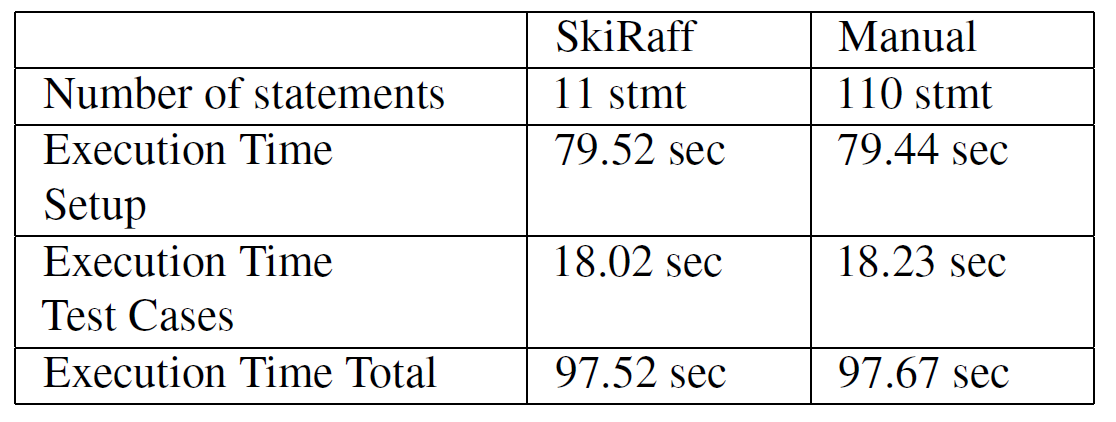
\includegraphics[width=1\textwidth]{figures/EvalResults.png}
        \caption{Results of evaluation, with 10000 rows in each table except for CountryDim}
        \label{Results of evaluation}
    \end{figure}
\end{frame}

\subsection{Alternativer}
\begin{frame}{Metrikker}{}
Statiske
  \begin{itemize}
    \item<1-> \textbf{Lines of code}
    \item<2-> Fog index
    \item<3-> Cyclomatic complexity
  	\end{itemize}

\pause
\pause
\pause
Dynamiske
  \begin{itemize}
    \item<4-> \textbf{Runtime}
    \item<5-> Bug Count
  	\end{itemize}
\end{frame}


\begin{frame}{Usability Testing}{}
Udførsel
  \begin{itemize}
    \item<1-> Opskriv flere realistiske test planer
    \item<2-> Få ekspert brugere til at implementere planer med forskellige værktøjer:
	 \begin{itemize}
   	 \item<2-> SkiRaff
    	\item<2-> Manuel
    	\item<2-> QuerySurge
	\item<2-> AnyDBTest
	\item<2-> Etc.
  	\end{itemize}
   \item<3-> Fokuser på implementations hastighed og udsagn
  	\end{itemize}

\pause
\pause
\pause
Negativer
 \begin{itemize}
   \item<4-> Praktisk organisering
    \item<5-> Kvalitativ data kan også være svær at evaluere
    \item<6-> Store mængder data skal behandles
  \end{itemize}
\end{frame}


\section{Conclusion}
\begin{frame}{Alexander}{}
  Hvad har vi lavet
  \begin{itemize}
    \item<1-> SkiRaff: Et framework til test af pygrametl programmer
    \item<2-> Dækker mange forskellige test cases med predicate klasserne
    \item<3-> Tests behøver færre linjer, men udføres med samme hastighed ift. manuel test
  \end{itemize}
\pause
\pause
\pause
Perspektiv
  \begin{itemize}
    \item<4-> Business Intelligence i moderne sammenhæng
    \item<5-> SkiRaff og agil udvikling
  \end{itemize}


\end{frame}


{\aauwavesbg
\begin{frame}[plain,noframenumbering]
  \finalpage{Thank you for listening}
\end{frame}}
%%%%%%%%%%%%%%%%

\end{document}
